\documentclass[11pt]{article}

\usepackage[T1]{fontenc}
\usepackage[utf8]{inputenc}
\usepackage{lmodern}

\usepackage{amsmath, amssymb, amsfonts, amsthm}
\usepackage{mathtools}

\usepackage{graphicx}
\usepackage{float}
\usepackage{booktabs}
\usepackage{array}
\usepackage{microtype}

\usepackage{hyperref}
\hypersetup{
  colorlinks=true,
  linkcolor=blue,
  citecolor=blue,
  urlcolor=blue
}

\usepackage{listings}
\lstset{
  basicstyle=\ttfamily\small,
  breaklines=true,
  frame=single,
  columns=fullflexible
}

% Optional: a simple boxed environment for callouts
\usepackage{mdframed}
\newmdenv[
  linewidth=0.6pt,
  roundcorner=6pt,
  innertopmargin=8pt,
  innerbottommargin=8pt,
  innerleftmargin=10pt,
  innerrightmargin=10pt
]{calloutnote}

% Bibliography (biblatex)
\usepackage[
  backend=biber,
  style=authoryear,
  maxcitenames=2,
  maxbibnames=99
]{biblatex}
\addbibresource{closed-form-fm-references.bib}

\title{Closed-Form Flow Matching: High-Dimensional Statistics and the Softmax Collapse}
\author{Nicolas Brosse}
\date{2025-12-10}

\begin{document}
\maketitle
\tableofcontents

Flow matching has emerged as a powerful framework for training continuous normalizing flows. In its Gaussian-OT instantiation, the \textbf{marginal velocity field} admits a closed form: it is a softmax-weighted average of per-example conditional velocities. In high dimension, a striking phenomenon occurs: the softmax weights become almost one-hot very early along the interpolation path. We refer to this as \textbf{softmax collapse}. It implies that the learned flow rapidly behaves like a nearest-neighbor map and tends to memorize the training set instead of sampling from the underlying data distribution.

In this post, building on the closed-form analysis of \cite{bertrand_closed-form_2025}, we study this collapse phenomenon through the lens of high-dimensional statistics and statistical physics. We view the softmax weights as a Gibbs measure over the training examples, with an energy that depends on the interpolation time $t$. This connects the behavior of flow matching to classic models such as the Random Energy Model (REM) and to Large Deviation Principles (LDP).

Our main goal is twofold:
\begin{enumerate}
\item \textbf{Mechanism.} Explain why, in high dimension, the marginal velocity field very quickly aligns with the conditional velocity field even for small $t$, and why neural networks find certain time regimes (around $t \approx 0.1$ and near $t \approx 1$) particularly hard to learn.
\item \textbf{Prediction.} Derive a \textbf{predictive formula for the collapse time}---the value of $t$ at which the softmax weights become essentially one-hot in a CIFAR-10 proxy.
\end{enumerate}

We adapt the dynamical and statistical-physics framework of \cite{biroli_dynamical_2024} to the flow-matching setting. Treating the softmax energies as REM-like random energies, we obtain an explicit asymptotic expression for the free energy, which in turn controls when the planted datapoint wins over all competing training samples. Specializing this analysis to a Gaussian proxy calibrated to CIFAR-10 yields a concrete collapse-time prediction.

\paragraph{Contributions}
\begin{itemize}
\item We interpret the closed-form marginal velocity field in flow matching as a Gibbs measure
\item Within an i.i.d.\ Gaussian toy model calibrated to CIFAR-10, we derive an explicit high-dimensional formula for the collapse time as a function of the dataset dimension, sample size, and variance, and give its numerical specialization for CIFAR-10.
\item We provide a self-contained, pedagogical derivation of the relevant LDP and REM results, aiming to be more accessible than \cite{bertrand_closed-form_2025} and to serve as a reference for readers interested in using these tools in generative modeling.
\end{itemize}

\noindent In Section~\ref{sec-setup-and-notation} we briefly recall the flow-matching and conditional flow-matching formulations and fix notation. In Section~\ref{sec-observations-on-the-marginal-velocity-field-conditional-velocity-field-and-training-difficulties}, we summarize the empirical behavior reported in \cite{bertrand_closed-form_2025}. Section~\ref{sec-cifar-10-preprocessing-and-statistics} justifies the Gaussian toy model used in the theory. The core statistical-physics analysis appears in Section~\ref{sec-marginal-velocity-field-collapse-a-statistical-physics-perspective}, and Section~\ref{sec-error-analysis-training-difficulties-across-time} connects the collapse picture back to the observed error profile of learned velocity fields. We include an accompanying notebook that numerically analyzes the CIFAR-10 dataset, computing both the collapse times and the correlation between the marginal and conditional velocity fields.

\section{Setup and Notation}\label{sec-setup-and-notation}
We follow the notation and setup of \cite[Section~2]{lipman_flow_2024} to present Flow Matching (FM). Given a training dataset with samples from an unknown target distribution $q$ over $\mathbb{R}^d$, the goal is to learn a model that can generate new samples from $q$. Flow Matching (FM) does this by defining a \textbf{continuous probability path} $(p_t)_{0\le t\le 1}$ that morphs a \textbf{known source distribution} $p_0=p$ (typically noise) into the \textbf{data distribution} $p_1=q$. FM learns a \textbf{time-dependent velocity field} $u_t$ (a vector field) that describes how samples move along this path. After training, sampling from $q$ works by:
\begin{enumerate}
\item Draw $X_0 \sim p$ (easy noise).
\item Solve an \textbf{ODE} driven by the learned velocity field to transport $X_0$ to $X_1$, which should follow $q$.
\end{enumerate}

FM uses a time-dependent vector field: $u : [0,1]\times \mathbb{R}^d \to \mathbb{R}^d$ and defines the associated \textbf{flow map} $\psi_t$ by the ODE:
\begin{equation}
\frac{d}{dt}\psi_t(x) = u_t(\psi_t(x)), \quad \psi_0(x)=x.
\end{equation}

If $u_t$ generates the probability path $p_t$, then pushing forward the source sample $X_0\sim p_0$ through the flow gives: $X_t := \psi_t(X_0) \sim p_t$. In particular, integrating to $t=1$ yields: $X_1=\psi_1(X_0) \approx q$. So the core objective is: \textbf{learn a neural velocity field} $u^\theta_t$ whose flow maps $p_0$ to $p_1$. Ideally, FM would minimize the mean-squared error between the learned and true velocity fields:
\begin{equation}
\mathcal{L}_{\text{FM}}(\theta)=\mathbb{E}_{t,X_t}\Big[\ \|u^\theta_t(X_t)-u_t(X_t)\|^2\ \Big],
\quad t\sim \mathcal{U}[0,1],\ X_t\sim p_t.
\end{equation}

But the marginal velocity field $u_t$ is usually hard to compute. Let the source be standard Gaussian: $p := p_0 = \mathcal{N}(0,I)$. A convenient path can be built by mixing \textbf{conditional paths} $p_{t|1}(x|x_1)$, each conditioned on a data example $X_1=x_1$. The resulting marginal path is:
\begin{equation}
p_t(x)=\int p_{t|1}(x|x_1) q(x_1) dx_1,
\quad\text{where}\quad
p_{t|1}(x|x_1)=\mathcal{N}\big(x\mid t x_1,\ (1-t)^2 I\big).
\end{equation}

A simple way to sample from this $p_t$ is:
\begin{equation}
X_t = tX_1 + (1-t)X_0 \sim p_t,
\end{equation}
where $X_0\sim p$ and $X_1\sim q$.

Condition on a randomly chosen training sample $X_1=x_1$ and define:
\begin{equation}
X_{t|1}=t x_1+(1-t)X_0 \sim p_{t|1}(\cdot|x_1).
\end{equation}
For this conditional Gaussian path, the ODE gives a \textbf{simple closed-form conditional velocity field}:
\begin{equation}
u_t(x|x_1)=\frac{x_1-x}{1-t}.
\end{equation}

This yields a tractable loss:
\begin{equation}
\mathcal{L}_{\text{CFM}}(\theta)=
\mathbb{E}_{t,X_t,X_1}\Big[\ \|u^\theta_t(X_t)-u_t(X_t|X_1)\|^2\ \Big],
\quad t\sim\mathcal{U}[0,1],\ X_0\sim p,\ X_1\sim q,
\end{equation}
with $X_t=(1-t)X_0+tX_1$. Crucially, this conditional objective provides the \textbf{same gradients} as the original FM loss:
\begin{equation}
\nabla_\theta \mathcal{L}_{\text{FM}}(\theta)=\nabla_\theta \mathcal{L}_{\text{CFM}}(\theta).
\end{equation}

Plugging the conditional velocity into the loss gives a common practical form:
\begin{equation}
\mathcal{L}^{\text{OT,Gauss}}_{\text{CFM}}(\theta)
= \mathbb{E}_{t,X_0,X_1}\Big[\ \|u^\theta_t(X_t)-(X_1-X_0)\|^2\ \Big],
\quad t\sim\mathcal{U}[0,1],\ X_0\sim\mathcal{N}(0,I),\ X_1\sim q,
\end{equation}
where $X_t=(1-t)X_0+tX_1$.

The CFM and FM losses are related by a bias-variance decomposition. The CFM loss can be written as:
\begin{equation}
\mathcal{L}_{\text{CFM}}(\theta) = \mathcal{L}_{\text{FM}}(\theta) + \mathbb{E}_{t, X_t}\left[\mathrm{Var}(X_1 - X_0 \mid X_t)\right].
\end{equation}

\begin{calloutnote}
\textbf{Proof of the loss decomposition.}

At the interpolant $X_t = (1-t)X_0 + tX_1$, the conditional velocity field evaluates to:
\begin{equation}
u_t(X_t \mid X_1) = \frac{X_1 - X_t}{1-t} = X_1 - X_0.
\end{equation}
The marginal velocity field at $X_t$ is the conditional expectation of this:
\begin{equation}
u_t(X_t) = \mathbb{E}[X_1 - X_0 \mid X_t].
\end{equation}
Let $Y = X_1 - X_0$ denote the target and $\bar{Y} = \mathbb{E}[Y \mid X_t] = u_t(X_t)$ the optimal predictor. We decompose:
\begin{equation}
\|u^\theta_t(X_t) - Y\|^2 = \|(u^\theta_t(X_t) - \bar{Y}) + (\bar{Y} - Y)\|^2.
\end{equation}
Expanding and taking the conditional expectation, the cross-term vanishes and we obtain the desired decomposition.
\end{calloutnote}

The second term is the \textbf{irreducible variance} --- it does not depend on $\theta$ and represents the inherent uncertainty in predicting the conditional velocity $X_1 - X_0$ from $X_t$ alone. This variance captures how much the target $X_1 - X_0$ fluctuates across different $(X_0, X_1)$ pairs that pass through the same interpolant $X_t$.

\section{Observations on the Marginal Velocity Field, Conditional Velocity Field and Training Difficulties}\label{sec-observations-on-the-marginal-velocity-field-conditional-velocity-field-and-training-difficulties}
In this section, we present some observations made in \cite{bertrand_closed-form_2025}. We focus on the case where the source distribution $p_0$ is the standard normal distribution and the data distribution $p_{\text{data}}$ is the CIFAR-10 dataset. We observe $n$ datapoints from CIFAR-10:
\begin{equation}
x^{(1)},\dots,x^{(n)} \sim p_{\text{data}}, \qquad x^{(i)}\in\mathbb{R}^d.
\end{equation}

In that scenario, we do not have access to the data distribution $p_{\text{data}}$, but only to the empirical distribution:
\begin{equation}\label{eq-empirical-distribution}
\hat p_{\text{data}}:=\frac1n\sum_{i=1}^n \delta_{x^{(i)}}.
\end{equation}

The marginal velocity field becomes available in closed form:
\begin{equation}
u_t(x) = \sum_{i=1}^n \lambda_i(x,t) \frac{x^{(i)} - x}{1-t},
\quad
\lambda_i(x,t)=\mathrm{softmax}\left(-\frac{\|x-t x^{(i)}\|^2}{2(1-t)^2}\right),
\end{equation}
where the softmax is taken over $i\in\{1, \dots, n\}$, i.e.
\begin{equation}
\lambda_i(x,t)=\frac{\exp\left(-\frac{\|x-t x^{(i)}\|^2}{2(1-t)^2}\right)}{\sum_{j=1}^n \exp\left(-\frac{\|x-t x^{(j)}\|^2}{2(1-t)^2}\right)}.
\end{equation}

\cite{bertrand_closed-form_2025} focuses on the memorization paradox, the fact that in that context with the empirical distribution \eqref{eq-empirical-distribution}, if the learning procedure outputs the marginal vector field, we recovers exactly the $n$ datapoints and not random samples from $p_{\text{data}}$.

In their study, they study the relation between the marginal velocity field available in closed form, the conditional velocity field and the empirical velocity field learned by a neural network. We focus on this aspect of their work.

They have 2 main observations:
\begin{enumerate}
\item As the dimension grows, the marginal velocity field is rapidly correlated (even when $t$ is very small) to the conditional velocity field.
\item The neural network has difficulties to learn the marginal velocity field for $t$ close to 0.1 and close to 1.
\end{enumerate}

We will expand on these observations in the next sections. The objective of this blog post is to provide some orders of magnitude of the softmax weights of the marginal velocity field, in particular in high dimension for CIFAR-10.

\begin{figure}[H]
\centering
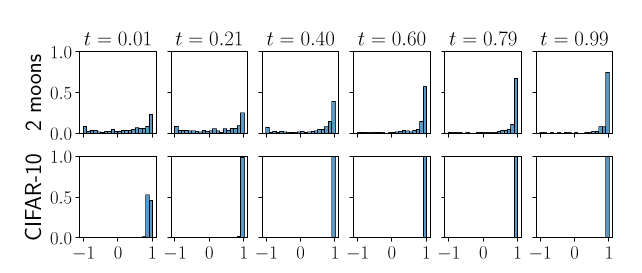
\includegraphics[width=\linewidth]{figures/article-fig-1.png}
\caption{The histograms of the cosine similarities between $u_t((1-t)x_0 + tx_1)$ and $u_t((1-t)x_0 + tx_1 \mid x_1) = x_1 - x_0$ are displayed for various time values $t$ and two datasets: 2-moons and CIFAR-10. \cite[Figure~1]{bertrand_closed-form_2025}}
\label{fig-article-fig-1}
\end{figure}

\begin{figure}[H]
\centering
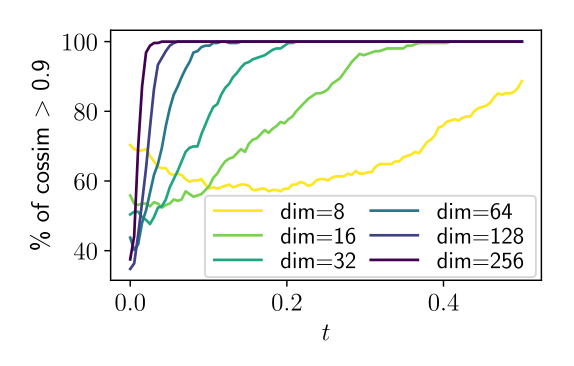
\includegraphics[width=\linewidth]{figures/article-fig-2.png}
\caption{Proportion of samples $x_t$ for which the cosine similarity between $u_t(x_t)$ and $u_t(x_t \mid x_1)$ exceeds 0.9, as a function of time $t$. This analysis is performed across multiple spatial resolutions of the Imagenette dataset, obtaining $d \times d$ images by spatial subsampling. \cite[Figure~2]{bertrand_closed-form_2025}}
\label{fig-article-fig-2}
\end{figure}

\begin{figure}[H]
\centering
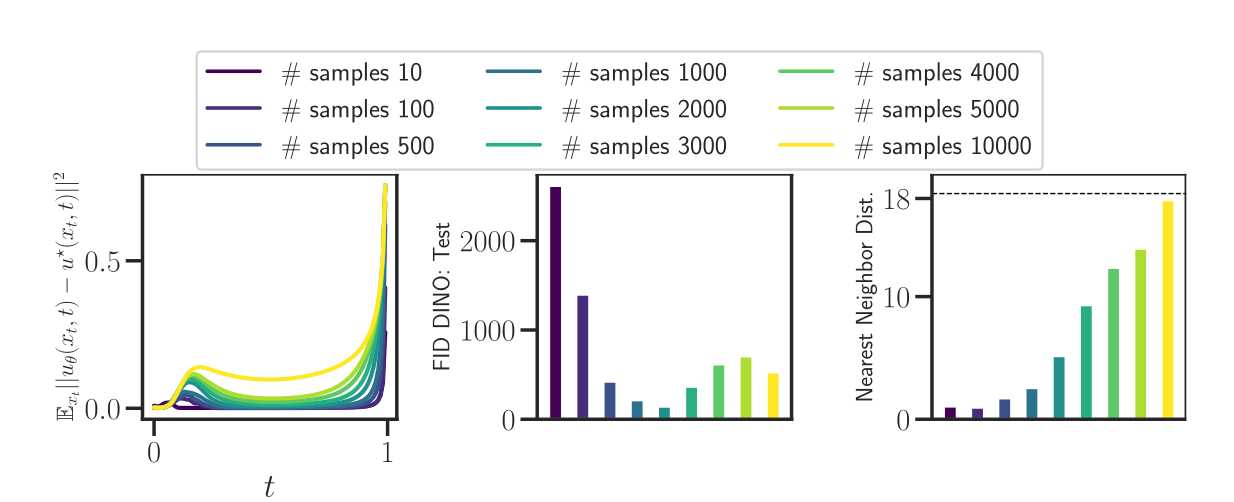
\includegraphics[width=\linewidth]{figures/article-fig-3.png}
\caption{Failure to learn the marginal velocity field on CIFAR-10: the leftmost figure represents the average error between the marginal empirical velocity field $u_t$ and the learned velocity $u^\theta_t$ for multiple values of time $t$. All the quantities are computed/learned on a varying number of training samples ($10$ to $10^4$) of the CIFAR-10 dataset. We are not interested in the other figures in this blog post. \cite[Figure~3]{bertrand_closed-form_2025}}
\label{fig-article-fig-3}
\end{figure}

\section{CIFAR-10 Preprocessing and Statistics}\label{sec-cifar-10-preprocessing-and-statistics}
We use standard CIFAR-10 preprocessing following the \href{https://github.com/atong01/conditional-flow-matching}{conditional-flow-matching} repository:
\begin{lstlisting}[language=Python]
dataset = datasets.CIFAR10(
    root="./data",
    train=True,
    download=True,
    transform=transforms.Compose([
        transforms.ToTensor(),
        transforms.Normalize((0.5, 0.5, 0.5), (0.5, 0.5, 0.5)),
    ]),
)
\end{lstlisting}

With \texttt{ToTensor()} (pixels in $[0,1]$) followed by normalization:
\begin{equation}
x = \frac{\text{pixel} - 0.5}{0.5} = 2 \cdot \text{pixel} - 1 \in [-1, 1].
\end{equation}

Each coordinate is bounded and roughly centered near 0. In high dimension, the vector behaves like a collection of weakly dependent coordinates.

\textbf{Key Parameters}
\begin{table}[H]
\centering
\begin{tabular}{@{}lll@{}}
\toprule
Parameter & Value & Description \\ \midrule
$d$ & $3 \times 32 \times 32 = 3072$ & Dimension \\
$\sigma^2$ & $\approx 0.24$ & Per-coordinate variance \\
$n$ & $50{,}000$ & Number of training samples \\ \bottomrule
\end{tabular}
\end{table}

A \href{https://github.com/kuangliu/pytorch-cifar/issues/19}{commonly cited computation} over the CIFAR-10 training set gives:
\begin{itemize}
\item mean $\approx (0.4914, 0.4822, 0.4465)$
\item std $\approx (0.247, 0.243, 0.261)$
\end{itemize}

(Those are for pixel values in $[0,1]$, i.e., after \texttt{ToTensor()}.)

With normalization by Torchvision, the variance transforms as $y = \frac{x - \mu}{\sigma}$ with $\mu=0.5$ and $\sigma=0.5$, so:
\begin{equation}
\mathrm{Var}(y) = \frac{\mathrm{Var}(x)}{\sigma^2} = \frac{\mathrm{Var}(x)}{0.25} = 4\,\mathrm{Var}(x).
\end{equation}

Using the CIFAR-10 channel stds above:
\begin{itemize}
\item $\mathrm{Var}(x_R) \approx 0.247^2 \approx 0.0610 \Rightarrow \mathrm{Var}(y_R)\approx 4\cdot 0.0610 \approx 0.244$
\item $\mathrm{Var}(x_G) \approx 0.243^2 \approx 0.0590 \Rightarrow \mathrm{Var}(y_G)\approx 0.236$
\item $\mathrm{Var}(x_B) \approx 0.261^2 \approx 0.0681 \Rightarrow \mathrm{Var}(y_B)\approx 0.273$
\end{itemize}

These are all of the same order, and for simplicity we use a representative value
\begin{equation}
\sigma^2 \approx 0.24
\end{equation}
for the per-coordinate variance of the normalized dataset.

\subsection{Remark: Channel Statistics vs. Pixel Statistics}
It is natural to ask how \textbf{channel-wise statistics} (mean and variance computed over all pixels in a given channel) relate to \textbf{per-pixel statistics} (mean and variance at a fixed spatial location).

Fix a channel (say, red) and let $X_{u,v}$ denote the intensity at pixel location $(u,v)$ for a random CIFAR-10 image. Let $(U,V)$ be a pixel location drawn uniformly at random from the grid, independently of the image, and define the ``global random pixel''
\begin{equation}
Y := X_{U,V}.
\end{equation}

By the law of total variance,
\begin{equation}
\mathrm{Var}(Y)= \mathbb{E}_{U,V}\bigl[\mathrm{Var}(X_{u,v})\bigr] + \mathrm{Var}_{U,V}\bigl(\mathbb{E}[X_{u,v}]\bigr).
\end{equation}

Interpreting the terms:
\begin{itemize}
\item $\mathbb{E}_{U,V}[\mathrm{Var}(X_{u,v})]$ is the \textbf{average per-pixel variance} (variance across images, averaged over spatial locations).
\item $\mathrm{Var}(Y)$ is the \textbf{global channel variance} when pooling all pixels in that channel.
\item The nonnegative term $\mathrm{Var}_{U,V}(\mathbb{E}[X_{u,v}])$ measures how much the \textbf{mean image} varies across spatial location.
\end{itemize}

Therefore,
\begin{equation}
\mathbb{E}_{U,V}\bigl[\mathrm{Var}(X_{u,v})\bigr] \le \mathrm{Var}(Y),
\end{equation}
and the gap is exactly the ``variance of the per-pixel means.''

On CIFAR-10, this spatial variation term is present (e.g., backgrounds vs. object centers) but is not typically huge compared to the intrinsic per-pixel variability. Hence:
\begin{itemize}
\item channel-level variances (like the CIFAR-10 stds above) and
\item average per-pixel variances
\end{itemize}
are of the \textbf{same order of magnitude}, with the global (pooled) variance usually slightly larger.

\subsection{Gaussian Toy Model and Its Limitations}\label{sec-gaussian-toy-model}
In the theoretical analysis below, we \textbf{idealize} the dataset as consisting of i.i.d. Gaussian vectors:
\begin{equation}
x_1, \dots, x_n \in \mathbb{R}^d,
\qquad
x_i \sim \mathcal{N}(0, \sigma^2 I_d),
\end{equation}
with
\begin{equation}
d = 3072,
\quad
n = 50{,}000,
\quad
\sigma^2 \approx 0.24.
\end{equation}
This model should be understood as a \textbf{toy approximation}: it preserves only very coarse statistics (dimension, scale of per-coordinate variance, approximate centering) and treats coordinates as independent and identically distributed.

Of course, real CIFAR-10 images are far from i.i.d. Gaussian vectors. The true covariance has a highly nontrivial structure, as illustrated by the empirical eigenvalue spectrum of the covariance matrix in Figure~\ref{fig-eigenvalues-cifar10}.

\begin{figure}[H]
\centering

\includegraphics[width=\linewidth]{figures/eigenvalues-cifar10.png}
\caption{The eigenvalues of the covariance matrix of the CIFAR-10 dataset.}
\label{fig-eigenvalues-cifar10}
\end{figure}

\noindent The pronounced decay and variability of eigenvalues in Figure~\ref{fig-eigenvalues-cifar10} reflect strong dependencies across pixels and channels (e.g., spatial correlation, global color structure, object/background patterns). The i.i.d. Gaussian model thus serves only as a \textbf{simplified reference}, not as a realistic generative model for CIFAR-10.

\section{Marginal Velocity Field Collapse: A Statistical Physics Perspective}\label{sec-marginal-velocity-field-collapse-a-statistical-physics-perspective}
This section provides a rigorous analysis of the collapse phenomenon in the marginal velocity field using tools from statistical physics, specifically the Random Energy Model (REM) and Large Deviation Principles (LDP).

\subsection{Gibbs Measure and Energy Formulation}
\subsubsection{The Marginal Velocity Field as a Gibbs Measure}
The marginal velocity field in Flow Matching is:
\begin{equation}
u_t(x) = \sum_{i=1}^n \lambda_i(x,t) \frac{x^{(i)} - x}{1-t},
\end{equation}
where
\begin{equation}
\lambda_i(x,t) = \frac{\exp\left(-\frac{\|x - tx^{(i)}\|^2}{2(1-t)^2}\right)}{\sum_{j=1}^n \exp\left(-\frac{\|x - tx^{(j)}\|^2}{2(1-t)^2}\right)}.
\end{equation}
This is a Boltzmann distribution at inverse temperature $\beta=1$ over states $i\in\{1,\dots,n\}$ with energy
\begin{equation}
E_i(x,t) = \frac{\|x - tx^{(i)}\|^2}{2(1-t)^2}.
\end{equation}
The denominator defines the partition function
\begin{equation}
Z(x,t) = \sum_{j=1}^n e^{-E_j(x,t)}.
\end{equation}

\subsubsection{Assumptions on the Data}
From Section~\ref{sec-gaussian-toy-model}, we consider a \textbf{Gaussian proxy} for the training data:
\begin{equation}
x^{(i)} \stackrel{\text{i.i.d.}}{\sim} \mathcal{N}(0, \sigma^2 I_d), \quad i = 1, \dots, n.
\end{equation}

This approximation captures the essential high-dimensional geometry while enabling analytical tractability. For CIFAR-10 after standard normalization, $\sigma^2 \approx 0.24$ provides a reasonable proxy.

\subsubsection{The ``Planted'' Trajectory}
Consider a trajectory starting from noise and targeting a specific training image:
\begin{equation}
x_t = (1-t)x_0 + tx_1, \quad x_0 \sim \mathcal{N}(0, I_d), \quad x_1 = x^{(1)}.
\end{equation}
Index $i=1$ is the planted index. For this index,
\begin{equation}
x_t - t x^{(1)} = (1-t) x_0,
\end{equation}
so the planted energy is
\begin{equation}
E_1(x_t,t) = \frac{\|(1-t)x_0\|^2}{2(1-t)^2} = \frac{\|x_0\|^2}{2}.
\end{equation}
By LLN for chi-squared variables,
\begin{equation}
\frac{E_1}{d} \xrightarrow{d\to\infty} \frac{1}{2} \quad \text{a.s.}
\end{equation}
Hence $Z_1=e^{-E_1}\approx e^{-d/2}$.

\subsubsection{The ``Bulk'' (REM-like) Energies}
For $j\neq 1$,
\begin{equation}
x_t - t x^{(j)} = (1-t)x_0 + t(x_1 - x^{(j)}).
\end{equation}
Under the Gaussian proxy, $x_1 - x^{(j)} \sim \mathcal{N}(0, 2\sigma^2 I_d)$ independent of $x_0$. Therefore
\begin{equation}
x_t - t x^{(j)} \sim \mathcal{N}(0, s^2(t) I_d), \quad s^2(t) := (1-t)^2 + 2\sigma^2 t^2.
\end{equation}
The bulk energies become
\begin{equation}
E_j(x_t,t)=\frac{\|x_t - t x^{(j)}\|^2}{2(1-t)^2}
\approx \frac{s^2(t)}{2(1-t)^2}\,\chi_d^2.
\end{equation}
Define the time-dependent energy scale
\begin{equation}
c(t) = \frac{s^2(t)}{2(1-t)^2}
= \frac{1}{2}\left(1 + \frac{2\sigma^2 t^2}{(1-t)^2}\right).
\end{equation}

\textbf{Key observation:} The bulk energies are approximately i.i.d. across $j \geq 2$, each extensive (order $d$). This is the classic setup where \textbf{Random Energy Model (REM)} tools apply.

Define the bulk partition function
\begin{equation}
Z_{\text{bulk}}(x,t) := \sum_{j=2}^n e^{-E_j(x,t)}.
\end{equation}
Following the statistical-physics convention, we call the normalized log of the bulk partition function the (quenched) \textbf{bulk free-energy density} at inverse temperature $\beta = 1$:
\begin{equation}
\Phi(1) := \lim_{d \to \infty} \frac{1}{d} \log Z_{\text{bulk}}(x_t,t),
\end{equation}
whenever the limit exists.

When we want to keep the time dependence explicit we will also write $\Phi(1,t)$.

\subsection{Collapsed vs Uncollapsed States (Glass vs Liquid)}
\subsubsection{Definition of Collapse}
The central question is whether the partition function $Z(x_t, t)$ is dominated by:
\begin{itemize}
\item \textbf{One special term} (the planted state), or
\item \textbf{Exponentially many comparable terms} (the bulk).
\end{itemize}

This leads to two phases:
\begin{center}
\begin{tabular}{@{}llll@{}}
\toprule
Phase & Statistical Physics & Flow Matching & Behavior \\ \midrule
\textbf{Collapsed} & Glass / Condensed & Memorization & $\lambda_1 \approx 1$ \\
\textbf{Uncollapsed} & Liquid & Generalization & Mass spread over many $j$'s \\ \bottomrule
\end{tabular}
\end{center}

\subsubsection{Glass Phase (Collapsed / Memorization)}
In the collapsed phase, $Z \approx Z_1 = e^{-E_1}$, meaning $\lambda_1 \approx 1$.

The marginal velocity field then reduces to:
\begin{equation}
u_t(x_t) \approx \frac{x^{(1)} - x_t}{1-t} = \frac{x_1 - x_t}{1-t} = x_1 - x_0.
\end{equation}

This is precisely the \textbf{conditional velocity field}. The marginal flow aligns perfectly with the teacher trajectory, leading to memorization of training data.

\subsubsection{Liquid Phase (Uncollapsed / Generalization)}
In the liquid phase, $Z \approx Z_{\text{bulk}} = \sum_{j=2}^n e^{-E_j}$, with mass distributed across many states.

The velocity field is a genuine mixture of directions toward different training points, enabling interpolation and generalization.

\subsubsection{The Phase Transition}
The transition between phases depends on:
\begin{itemize}
\item \textbf{Energy advantage} of the planted state (order $d$)
\item \textbf{Entropy} from having $n$ competitors (order $\log n$)
\end{itemize}

The competition is controlled by the \textbf{dimensionless ratio}:
\begin{equation}
\alpha = \frac{\log n}{d}.
\end{equation}

For typical datasets (e.g., CIFAR-10 with $d = 3072$, $n = 50{,}000$):
\begin{equation}
\alpha = \frac{\log(50{,}000)}{3072} \approx 0.0035 \ll 1.
\end{equation}

This tiny $\alpha$ means the entropy budget is negligible compared to extensive energy gaps, placing the system deep in the collapsed regime for most values of $t$.

\subsection{Simple Heuristic Analysis}
\subsubsection{Typical Energy Gap}
Compare a typical bulk energy to the planted energy. The \textbf{typical energy gap} is:
\begin{align}
E_j - E_1
&\approx \frac{d}{2}\left(\frac{s^2(t)}{(1-t)^2}-1\right)
= \frac{d}{2}\cdot \frac{2\sigma^2 t^2}{(1-t)^2}
= \frac{d\sigma^2 t^2}{(1-t)^2}.
\end{align}

Therefore, the log-weight ratio is:
\begin{equation}
\log\frac{\lambda_j}{\lambda_1}\approx -(E_j-E_1)\approx -\frac{d\sigma^2 t^2}{(1-t)^2},
\end{equation}
showing \textbf{exponential-in-$d$ suppression} of bulk weights relative to the planted weight.

\subsubsection{Crude Annealed Entropy Estimate}
A naive estimate of the bulk partition function uses the \textbf{annealed approximation}:
\begin{equation}
Z_{\text{bulk}} \approx (n-1) \cdot \mathbb{E}[e^{-E_j}].
\end{equation}

However, this is often wrong because $e^{-E_j}$ has exponentially broad fluctuations. The sum is dominated by \textbf{rare low-energy states}, not typical ones. This is precisely where REM physics becomes essential.

\subsubsection{Energy vs Entropy Competition}
The competition can be summarized as:
\begin{itemize}
\item \textbf{Planted contribution:} $Z_1 \sim e^{-d/2}$
\item \textbf{Bulk contribution (naive):} $Z_{\text{bulk}} \sim n \cdot e^{-d \cdot c(t)} = e^{\alpha d - d \cdot c(t)}$
\end{itemize}

For the planted state to dominate, we need the energy advantage to exceed the entropy:
\begin{equation}
\frac{d \sigma^2 t^2}{(1-t)^2} \gg \log n.
\end{equation}

Rearranging, collapse holds whenever:
\begin{equation}
\frac{t}{1-t} \gg \sqrt{\frac{\log n}{d \sigma^2}}.
\end{equation}

For CIFAR-like numbers, the right-hand side is tiny ($\approx 0.12$), so collapse can occur at small $t$.

\subsubsection{Simple Collapse Time Estimate}
Setting the two sides equal gives a heuristic collapse time:
\begin{equation}
t_C^{\text{heuristic}} \approx \frac{\sqrt{\alpha/\sigma^2}}{1 + \sqrt{\alpha/\sigma^2}}.
\end{equation}

For CIFAR-10 ($\alpha \approx 0.0035$, $\sigma^2 \approx 0.24$):
\begin{equation}
t_C^{\text{heuristic}} \approx 0.11.
\end{equation}

\textbf{Caveat:} This estimate compares typical bulk energy to planted energy. A rigorous analysis must consider the \textbf{best} competitor among $n-1$ states, not a typical one. This requires REM/LDP tools.

\subsection{Rigorous REM/LDP Derivation}
\subsubsection{Large Deviation Principles: Foundations}
\paragraph{Why LDP?}
The Law of Large Numbers tells us \emph{where} random variables concentrate, but not \emph{how unlikely} deviations are. Large Deviation Theory provides \textbf{exponential decay rates} for rare events.

\paragraph{Definition}
A sequence of random variables $X_d$ satisfies a \textbf{Large Deviation Principle (LDP)} with rate function $I(x)$ if:
\begin{equation}
\mathbb{P}(X_d \approx x) \asymp e^{-d \, I(x)}
\end{equation}
where:
\begin{itemize}
\item $d$ is the large parameter (dimension)
\item $I(x) \geq 0$ with $I(x) = 0$ at the typical value
\item larger $I(x)$ means exponentially rarer events
\end{itemize}

\paragraph{Cram\'er's Theorem}
For i.i.d.\ random variables $X_1, \dots, X_d$ with finite moment generating function, the empirical average $S_d = \frac{1}{d}\sum_{k=1}^d X_k$ satisfies an LDP:
\begin{equation}
\mathbb{P}(S_d \approx x) \asymp e^{-d \, I(x)}
\end{equation}
where the \textbf{rate function} is the Legendre transform of the log-MGF:
\begin{equation}
I(x) = \sup_{\lambda \in \mathbb{R}} \left( \lambda x - \log \mathbb{E}[e^{\lambda X_1}] \right).
\end{equation}

\subsubsection{LDP for Chi-Squared (Energy Density)}
\paragraph{Deriving the Rate Function}
Let $Z_k \sim \mathcal{N}(0,1)$ i.i.d., so $\chi_d^2 = \sum_{k=1}^d Z_k^2$. Define:
\begin{equation}
Y_d = \frac{\chi_d^2}{d} = \frac{1}{d}\sum_{k=1}^d Z_k^2.
\end{equation}

For $X = Z^2$, the log-MGF is:
\begin{equation}
\log \mathbb{E}[e^{\lambda Z^2}] = -\frac{1}{2}\log(1 - 2\lambda), \quad \lambda < \frac{1}{2}.
\end{equation}

Applying Cram\'er's theorem and computing the Legendre transform:
\begin{equation}
I_\chi(y) = \sup_{\lambda < 1/2}\left(\lambda y + \frac{1}{2}\log(1 - 2\lambda)\right) = \frac{1}{2}(y - 1 - \log y), \quad y > 0.
\end{equation}

\textbf{Key properties:}
\begin{itemize}
\item minimum at $y = 1$ with $I_\chi(1) = 0$ (typical value)
\item convex and non-negative
\item deviations are exponentially unlikely in $d$
\end{itemize}

\paragraph{Energy Density LDP}
For bulk energies with $E = c(t) \cdot \chi_d^2$, the energy density $e = E/d = c \cdot Y_d$ satisfies:
\begin{equation}
\mathbb{P}(e \approx \varepsilon) \asymp e^{-d \, I(\varepsilon)}
\end{equation}
where:
\begin{equation}
\boxed{
I(\varepsilon) = \frac{1}{2}\left(\frac{\varepsilon}{c} - 1 - \log\frac{\varepsilon}{c}\right)
}
\end{equation}

This is the \textbf{rigorous backbone} for all REM arguments.

\subsubsection{Bulk Free Energy via Laplace Principle}
\paragraph{Complexity (Entropy of States)}
With $n = e^{\alpha d}$ bulk energies, the expected \textbf{number of states} with energy density near $\varepsilon$ is:
\begin{equation}
\#(\varepsilon) \approx n \cdot \mathbb{P}(e \approx \varepsilon) \approx \exp\{d(\alpha - I(\varepsilon))\}.
\end{equation}

The quantity:
\begin{equation}
\Sigma(\varepsilon) = \alpha - I(\varepsilon)
\end{equation}
is the \textbf{complexity} (entropy density of states at energy $\varepsilon$).

\paragraph{Laplace Principle}
The bulk partition function is approximately:
\begin{equation}
Z_{\text{bulk}} = \sum_{j=2}^n e^{-E_j} \approx \int d\varepsilon \, \exp\{d(\Sigma(\varepsilon) - \varepsilon)\}.
\end{equation}

Using the LDP for the bulk energies, the bulk free-energy density $\Phi(1)$ defined above can be computed via a Laplace (saddle-point) principle:
\begin{equation}
\boxed{
\Phi(1) = \sup_{\varepsilon > 0}\left[\alpha - I(\varepsilon) - \varepsilon\right]
}
\end{equation}

\subsubsection{Glass vs Liquid Phase Transition}
\paragraph{The Variational Problem}
Define $F(\varepsilon) = \alpha - I(\varepsilon) - \varepsilon$. The maximizer determines the phase.

\paragraph{Liquid Phase (Interior Solution)}
If the maximizer is interior, it satisfies $F'(\varepsilon) = 0$, i.e., $I'(\varepsilon) = -1$.

Computing:
\begin{equation}
I'(\varepsilon) = \frac{1}{2}\left(\frac{1}{c} - \frac{1}{\varepsilon}\right) = -1
\end{equation}

yields the \textbf{liquid saddle point}:
\begin{equation}
\boxed{\varepsilon_* = \frac{c}{1 + 2c}}
\end{equation}

This solution is valid only if there are exponentially many states there: $\Sigma(\varepsilon_*) = \alpha - I(\varepsilon_*) \geq 0$.

\paragraph{Glass Phase (Boundary Solution)}
If $\alpha - I(\varepsilon_*) < 0$, there are too few states at the liquid saddle. The supremum hits the boundary where complexity vanishes:
\begin{equation}
I(\varepsilon_g) = \alpha
\end{equation}

The partition sum is then dominated by the \textbf{lowest-energy extremes}: this is the glass/condensed phase.

\paragraph{Freezing Threshold}
The critical entropy level separating phases is:
\begin{equation}
\boxed{\alpha_c(c) = I(\varepsilon_*) = \frac{1}{2}\left(\log(1 + 2c) - \frac{2c}{1 + 2c}\right)}
\end{equation}

\textbf{Phase diagram:}
\begin{itemize}
\item \textbf{Liquid phase:} $\alpha \geq \alpha_c(c)$, maximizer at $\varepsilon_*$, free energy $\Phi(1) = \alpha - I(\varepsilon_*) - \varepsilon_*$
\item \textbf{Glass phase:} $\alpha < \alpha_c(c)$, maximizer at $\varepsilon_g$ with $I(\varepsilon_g) = \alpha$, free energy $\Phi(1) = -\varepsilon_g$
\end{itemize}

\subsubsection{Collapse Criterion from Free Energy}
\paragraph{Full Partition Function}
The complete partition function is:
\begin{equation}
Z = e^{-E_1} + Z_{\text{bulk}}, \quad \lambda_1 = \frac{e^{-E_1}}{Z}.
\end{equation}

Since $E_1/d \to 1/2$, we have:
\begin{equation}
\frac{1}{d}\log\frac{Z_{\text{bulk}}}{e^{-E_1}} \to \Phi(1) + \frac{1}{2}.
\end{equation}

\paragraph{Collapse Condition}
\begin{equation}
\boxed{\lambda_1 \to 1 \iff \Phi(1) < -\frac{1}{2}}
\end{equation}

More precisely, for large $d$:
\begin{equation}
\lambda_1 \approx \frac{1}{1 + \exp\{d(\Phi(1) + 1/2)\}}.
\end{equation}

\paragraph{Glass Phase Collapse Criterion}
In the glass phase, $\Phi(1) = -\varepsilon_g$, so collapse requires:
\begin{equation}
\boxed{-\varepsilon_g < -\frac{1}{2} \iff \varepsilon_g > \frac{1}{2}}
\end{equation}
where $\varepsilon_g$ is defined implicitly by $I(\varepsilon_g) = \alpha$.

\textbf{Interpretation:} Collapse occurs when even the \emph{best} spurious competitor (with energy density $\varepsilon_g$) has higher energy than the planted state (energy density $1/2$).

\paragraph{Liquid Phase Collapse Criterion}
In the liquid phase, collapse requires:
\begin{equation}
\alpha - I(\varepsilon_*) - \varepsilon_* < -\frac{1}{2}.
\end{equation}

This gives an explicit inequality in $c$ and $\alpha$.

\subsubsection{Explicit Collapse Time}
\paragraph{Collapse Time Equation}
The collapse time $t_C$ is defined by $\varepsilon_g(t_C) = 1/2$. Setting $\varepsilon_g = 1/2$ in $I(\varepsilon_g) = \alpha$:
\begin{equation}
\alpha = I(1/2) = \frac{1}{2}\left(\frac{1/2}{c} - 1 - \log\frac{1/2}{c}\right) = \frac{1}{2}\left(\frac{1}{2c} - 1 + \log(2c)\right).
\end{equation}

This gives the \textbf{REM-rigorous collapse boundary}:
\begin{equation}
\boxed{\alpha = \frac{1}{2}\left(\log(2c(t_C)) + \frac{1}{2c(t_C)} - 1\right)}
\end{equation}

with $c(t) = \frac{1}{2}\left(1 + \frac{2\sigma^2 t^2}{(1-t)^2}\right)$.

\paragraph{CIFAR-10 Proxy Calculation}
For CIFAR-10: $d = 3072$, $n = 50{,}000$, $\sigma^2 = 0.24$.

Compute:
\begin{equation}
\alpha = \frac{\log(50{,}000)}{3072} \approx 0.003522.
\end{equation}

Solving the collapse equation yields:
\begin{equation}
\boxed{t_C \approx 0.341}
\end{equation}

with corresponding $c(t_C) \approx 0.5644$.

\textbf{Interpretation:} Under the i.i.d. Gaussian proxy + REM idealization, for $t \lesssim 0.34$, the planted datapoint is no longer guaranteed to dominate because among $n$ training points, one can typically find at least one spurious point whose energy matches or beats the planted energy. For $t \gtrsim 0.34$, collapse occurs and the planted state dominates.

\paragraph{Why CIFAR is Always in the Glass Phase}
For CIFAR-like $\alpha \ll 1$, we have $\alpha \ll \alpha_c(c(t))$ for all $t \in [0,1)$. The system is \textbf{always in the glass phase}, meaning that the bulk partition function is dominated by a few extreme low-energy states.

\subsubsection{Summary of Key Equations}
\paragraph{Bulk Energy LDP}
\begin{equation}
\mathbb{P}\left(\frac{E}{d}\approx \varepsilon\right)\asymp e^{-d\,I(\varepsilon)},
\qquad
I(\varepsilon)=\frac{1}{2}\left(\frac{\varepsilon}{c}-1-\log\frac{\varepsilon}{c}\right).
\end{equation}

\paragraph{Bulk Quenched Free Energy}
\begin{equation}
\Phi(1) = \sup_{\varepsilon > 0}\left[\alpha - I(\varepsilon) - \varepsilon\right], \quad \alpha = \frac{\log n}{d}.
\end{equation}

\paragraph{Glass vs Liquid Threshold}
\begin{equation}
\alpha_c(c)=\frac{1}{2}\left(\log(1+2c)-\frac{2c}{1+2c}\right).
\end{equation}

\paragraph{Collapse Criterion}
\begin{equation}
\lambda_1 \to 1 \iff \Phi(1) < -\frac{1}{2}
\end{equation}
In the glass phase ($\alpha<\alpha_c$):
\begin{equation}
\lambda_1 \to 1 \iff \varepsilon_g > \frac{1}{2}, \quad I(\varepsilon_g) = \alpha
\end{equation}

\paragraph{Collapse Time (Glass Phase)}
\begin{equation}
\alpha=\frac{1}{2}\left(\log(2c(t_C))+\frac{1}{2c(t_C)}-1\right).
\end{equation}

\subsection{Extension to Non-Isotropic Covariance}
\subsubsection{Motivation}
The isotropic Gaussian proxy $x^{(i)} \sim \mathcal{N}(0, \sigma^2 I_d)$ is convenient but unrealistic. Real image datasets have structured covariance with varying eigenvalues (some directions have high variance, others low). The REM/LDP framework extends naturally to non-isotropic covariance. The structure of the theory remains identical --- only the \textbf{rate function} $I(\varepsilon)$ changes.

\subsubsection{Setup: General Covariance Model}
Assume training images follow:
\begin{equation}
x^{(i)} \sim \mathcal{N}(0, C), \quad i = 1, \dots, n
\end{equation}

\subsubsection{Deriving the Effective Covariance}
Let $C=U\operatorname{diag}(\mu_1,\dots,\mu_d)U^\top$ be an eigendecomposition.

For $j \ge 2$,
\begin{equation}
x_t - t x^{(j)} = (1-t)x_0 + t(x_1 - x^{(j)}),
\end{equation}
and since $x_0 \sim \mathcal{N}(0,I_d)$ and $x_1 - x^{(j)} \sim \mathcal{N}(0,2C)$ independent, we get
\begin{equation}
\operatorname{Cov}(x_t - t x^{(j)}) = (1-t)^2 I_d + 2t^2 C =: \Sigma_t.
\end{equation}

Let $g \sim \mathcal{N}(0,I_d)$, then $x_t - t x^{(j)} \overset{d}{=} \Sigma_t^{1/2} g$ and
\begin{equation}
E_j = \frac{g^\top \Sigma_t g}{2(1-t)^2} = \frac{1}{2}g^\top C_t g,
\qquad
C_t = \frac{\Sigma_t}{(1-t)^2} = I_d + \frac{2t^2}{(1-t)^2}C.
\end{equation}

\subsubsection{Eigenvalues of the Effective Covariance}
If $C$ has eigenvalues $\mu_k$, then $C_t$ has eigenvalues
\begin{equation}
\lambda_k^{(t)} = 1 + \frac{2t^2}{(1-t)^2}\mu_k, \qquad k=1,\dots,d.
\end{equation}

The bulk energy density is
\begin{equation}
\frac{E_j}{d} = \frac{1}{2d}\sum_{k=1}^d \lambda_k^{(t)} Z_k^2,
\qquad Z_k \sim \mathcal{N}(0,1) \ \text{i.i.d.}
\end{equation}

\textbf{Recovery of isotropic case:} When $C = \sigma^2 I_d$, all $\mu_k = \sigma^2$, so:
\begin{equation}
\lambda_k^{(t)} = 1 + \frac{2\sigma^2 t^2}{(1-t)^2} = 2c(t)
\end{equation}
which matches our earlier formula (the factor of 2 accounts for the $1/2$ in $E_j = \frac{1}{2}g^\top C_t g$).

\subsubsection{LDP for Weighted Chi-Squared: G\"artner-Ellis Theorem}
In the general covariance case, the energy density is a weighted sum of chi-squared variables:
\begin{equation}
\frac{E_j}{d} = \frac{1}{2d}\sum_{k=1}^d \lambda_k^{(t)} Z_k^2,
\end{equation}

a sum of independent but \textbf{non-identically distributed} terms (the weights $\lambda_k^{(t)}$ vary with $k$). To obtain an LDP in this heterogeneous setting, we use the \textbf{G\"artner--Ellis theorem}, which handles such triangular arrays via the limit of the log-moment generating function.

\textbf{Step 1: Compute the scaled cumulant generating function}

For a single term $\lambda Z^2$ with $Z \sim \mathcal{N}(0,1)$:
\begin{equation}
\mathbb{E}[e^{\theta \lambda Z^2}] = \frac{1}{\sqrt{1 - 2\theta\lambda}}, \quad \theta < \frac{1}{2\lambda}.
\end{equation}
Thus:
\begin{equation}
\log \mathbb{E}[e^{\theta \lambda Z^2}] = -\frac{1}{2}\log(1 - 2\theta\lambda).
\end{equation}

\textbf{Step 2: Sum over all eigenvalues}

The scaled log-MGF for the energy density $e = E_j/d$ is:
\begin{equation}
\Lambda_t(\theta) = \lim_{d \to \infty} \frac{1}{d} \log \mathbb{E}\left[e^{d\theta \cdot \frac{1}{2d}\sum_k \lambda_k^{(t)} Z_k^2}\right] = \lim_{d \to \infty} \frac{1}{d} \sum_{k=1}^d \left(-\frac{1}{2}\log\left(1 - \theta\lambda_k^{(t)}\right)\right).
\end{equation}

This limit exists if the \textbf{empirical spectral distribution} of $C_t$ converges:
\begin{equation}
\Lambda_t(\theta) = \int \left(-\frac{1}{2}\log(1 - \theta\lambda)\right) d\nu_t(\lambda)
\end{equation}
where $\nu_t$ is the limiting spectral measure of $\{\lambda_k^{(t)}\}$.

\textbf{Step 3: Legendre transform gives the rate function}

By the G\"artner--Ellis theorem:
\begin{equation}
\boxed{I_t(\varepsilon) = \sup_{\theta < 1/\lambda_{\max}^{(t)}} \left(\theta\varepsilon - \Lambda_t(\theta)\right)}
\end{equation}

This is the \textbf{drop-in replacement} for the isotropic rate function.

\subsubsection{The Full Pipeline with General Covariance}
The REM framework carries through unchanged:
\begin{enumerate}
\item \textbf{Bulk free energy:}
\begin{equation}
\Phi(1,t) = \sup_{\varepsilon > 0}\left[\alpha - I_t(\varepsilon) - \varepsilon\right]
\end{equation}
\item \textbf{Collapse criterion:}
\begin{equation}
\lambda_1 \to 1 \iff \Phi(1,t) < -\frac{1}{2}
\end{equation}
\item \textbf{Planted weight approximation:}
\begin{equation}
\lambda_1(t) \approx \frac{1}{1 + \exp\{d(\Phi(1,t) + 1/2)\}}
\end{equation}
\end{enumerate}

\noindent Only $I_t(\varepsilon)$ changes --- the rest of the theory is identical.

\section{Error Analysis: Training Difficulties Across Time}\label{sec-error-analysis-training-difficulties-across-time}
As observed in Figure~\ref{fig-article-fig-3}, the learned velocity field $u^\theta_t$ exhibits a characteristic error profile when approximating the marginal velocity field $u_t$: low error near $t = 0$, a peak around $t \approx 0.1$, a decrease for intermediate $t$, and a final spike near $t = 1$. This section tries to explain these four regimes.

\subsection{Training Error Trajectory: Four Regimes}
\subsubsection{Regime 1: $t \approx 0$ --- Trivial Learning Phase}
For small $t$, the interpolant is dominated by noise: $X_t = (1-t)X_0 + tX_1 \approx X_0$. The marginal velocity field at $X_t$ is:
\begin{equation}
u_t(X_t) = \frac{\mathbb{E}[X_1 \mid X_t] - X_t}{1-t}.
\end{equation}

When $t \approx 0$, the interpolant $X_t \approx X_0$ carries almost no information about $X_1$. Under the empirical distribution, the posterior mean satisfies:
\begin{equation}
\mathbb{E}[X_1 \mid X_t] \approx \bar{x} \approx 0
\end{equation}
where $\bar{x}$ is the mean of the training data (approximately zero after normalization).

Therefore, the optimal velocity field simplifies to:
\begin{equation}
u_t(X_t) \approx \frac{0 - X_t}{1-t} \approx \frac{-X_t}{1} = -X_t.
\end{equation}

This is essentially a \textbf{negation map}: the neural network only needs to learn $u^\theta_t(x) \approx -x$, which is trivial.

\subsubsection{Regime 2: $t \approx t_C$ --- Peak Difficulty (Collapse Transition)}
The error peaks around $t \approx 0.1$--$0.2$, which corresponds to the approach toward the \textbf{collapse transition} at $t_C$.

In this regime, the posterior $p(X_1 \mid X_t)$ is \textbf{neither uniform nor concentrated}:
\begin{itemize}
\item The interpolant $X_t$ now contains some information about $X_1$, so the posterior is no longer uniform over training points.
\item But collapse has not yet occurred, so multiple training points still have significant posterior weight.
\end{itemize}

This creates several sources of difficulty:
\begin{enumerate}
\item \textbf{Complex posterior structure:} The neural network must learn to predict $\mathbb{E}[X_1 \mid X_t]$, which is a weighted average over multiple training points. The weights $\lambda_i(X_t, t)$ vary rapidly with $X_t$.
\item \textbf{Signal-to-noise transition:} The interpolant $X_t = (1-t)X_0 + tX_1$ is transitioning from noise-dominated to signal-dominated. The network must extract $X_1$ from $X_t$, but $X_t$ is still far from $X_1$.
\item \textbf{Sharp phase transition:} The REM analysis shows that the energy gaps scale as:
\begin{equation}
E_j - E_1 \approx \frac{d \sigma^2 t^2}{(1-t)^2}.
\end{equation}

Near $t_C$, the system transitions from having exponentially many competing states to a single dominant state. This transition is sharp in high dimensions, creating rapid variation in the velocity field as a function of both $x$ and $t$.
\item \textbf{High sensitivity:} Near the transition, the map $x \mapsto \arg\max_i \lambda_i(x,t)$ is extremely sensitive to perturbations. Small changes in $X_t$ can cause different training points to dominate the posterior.
\end{enumerate}

\subsubsection{Regime 3: $t > t_C$ --- Decreasing Error (Concentration)}
After the collapse transition ($t > t_C$), the error \textbf{decreases}. The posterior concentrates on the planted index with $\lambda_1(X_t, t) \approx 1$.

In this regime:
\begin{equation}
u_t(X_t) \approx \frac{x^{(1)} - X_t}{1-t} = \frac{X_1 - X_t}{1-t} = X_1 - X_0.
\end{equation}

The marginal velocity field becomes essentially equal to the \textbf{conditional velocity field}. The neural network's task simplifies: given $X_t$, it must predict $X_1 - X_0$, but now $X_t$ strongly determines which $X_1$ generated it.

The learning problem has two favorable properties:
\begin{enumerate}
\item \textbf{Low posterior uncertainty:} With $\lambda_1 \approx 1$, there is little ambiguity about which training point generated $X_t$.
\item \textbf{Increasing signal:} As $t$ grows, $X_t$ becomes closer to $X_1$, making it easier to infer the target direction $X_1 - X_0$.
\end{enumerate}

Geometrically, the velocity field becomes piecewise-affine: within each Voronoi cell (determined by proximity to training points), the network must approximate
\begin{equation}
\frac{x^{(i)} - x}{1-t},
\end{equation}

where $i$ indexes the training point whose cell contains $x$. Although the coefficient $1/(1-t)$ grows as $t$ increases, the key simplification is that the posterior has collapsed---the network no longer faces the challenge of averaging over multiple competing directions.

\subsubsection{Regime 4: $t \to 1$ --- Final Blow-Up}
Near $t = 1$, the error spikes again due to \textbf{Voronoi discontinuities}.

\paragraph{Voronoi Discontinuities (Nearest-Neighbor Regime)}
As $t \to 1$, the softmax temperature $(1-t)^2 \to 0$ drives the weights toward a \textbf{one-hot distribution}:
\begin{equation}
\lambda_i(x,t) \xrightarrow{t \to 1} \mathbf{1}\left[i = \arg\min_j \|x - x^{(j)}\|\right].
\end{equation}

The marginal velocity field approaches:
\begin{equation}
u_t(x) \approx \frac{x^{(i^*)} - x}{1-t}, \quad \text{where } i^* = \arg\min_j \|x - x^{(j)}\|.
\end{equation}

This is a \textbf{piecewise-affine vector field} that switches abruptly across \textbf{Voronoi cell boundaries} in $\mathbb{R}^d$. Such discontinuous fields are notoriously difficult to approximate with smooth neural networks, explaining the error spike near $t \approx 1$.

\subsection{Summary: Error Profile Across Time}
\begin{center}
\begin{tabular}{@{}llll@{}}
\toprule
Regime & Time & Error & Explanation \\ \midrule
1 & $t \approx 0$ & Low & Posterior mean $\approx 0$; target is $\approx -X_0$ (trivial) \\
2 & $t \approx t_C$ & \textbf{Peak} & Complex posterior; phase transition; high sensitivity \\
3 & $t > t_C$ & Decreasing & Posterior concentrates; clear signal; simpler target structure \\
4 & $t \to 1$ & \textbf{Spike} & Voronoi discontinuities; $1/(1-t)$ blow-up \\ \bottomrule
\end{tabular}
\end{center}

\noindent \textbf{Accompanying notebook:} \texttt{notebooks/\_cifar10\_numerical\_analysis.ipynb}

\section{Conclusion}
Flow matching with Gaussian-OT admits a closed-form expression for the marginal velocity field: a softmax over the training examples. In high dimensions, this softmax typically \textbf{collapses} early, assigning nearly all weight to a single training point. As a result, the flow effectively implements a nearest-neighbor mapping and tends to memorize the dataset.

By representing CIFAR-10 data with a Gaussian proxy and leveraging techniques from the REM and LDP frameworks, we model the softmax weights as a Gibbs distribution and analyze the competition between the true (planted) data point and all others. This leads to an explicit, high-dimensional prediction of the \textbf{collapse time} ($t_C$), which is found to be surprisingly small for realistically sized CIFAR-10 data.

This analysis clarifies the characteristic error profile: neural networks struggle most at intermediate $t$ (near the collapse transition), and again as $t \to 1$ (where the velocity field develops Voronoi-type discontinuities), but not at small $t$. Softmax collapse thus emerges as a fundamental, high-dimensional property of the Gaussian-OT path---rather than merely an artifact of optimization---and should be deliberately considered in the design and training of flow-matching models.

\printbibliography

\end{document}
